\section{Conception}

\subsection{Introduction}
The idea of our project is as follows: \\ 
We wanted to come up with an easy way to check whether you have melanoma or not, without the need to go to a doctor, or you can use it as a second confirmation before or after you go to a dermatologist. And what is easier than a web application that you can access from anywhere and at anytime.

Our product can be used in 2 scenarios. Either by normal persons that are suspicious of having melanoma, they can use the application to decide whether to go to a dermatologist for further testing and confirmation. The second scenario is the use of this application by doctors to help them in the diagnosis process without having to do a lot of testing just to get initial results, you can think of the application as the replacement of the doctor's naked eye analysis, and after that he/she can decide whether to do more extensive testing such as biopsies. And as an added feature every user of the application can decide whether or not to publish his lesion image, which will then be accessible to all the doctors inside the application, and they can comment on it and give their professional opinion, after that the user can communicate with a doctor using the in-application messaging feature, to get more information or to make an appointment

In the next sections, we are going to present a set of diagrams that will explain the design of our web-based platform for skin cancer diagnosis.

\subsection{Class Diagram}
Class diagrams may be used to represent the system's constituent parts, show the connections between them, and offer information on the functions and services each one of them performs. The system design process benefits from class diagrams at various phases.

\begin{figure}[H]
\begin{center}
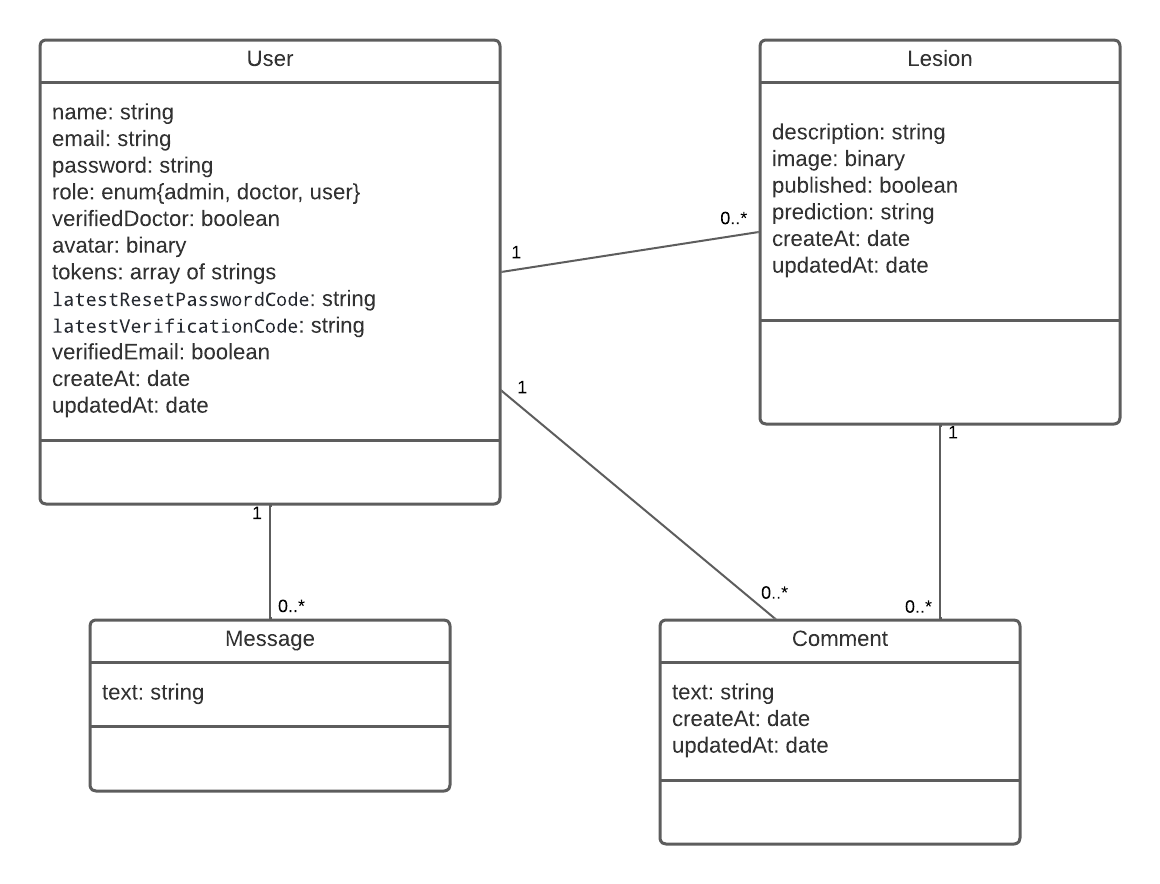
\includegraphics[width=12cm]{./diagnosis-system/conception/class.png}
\end{center}
\caption{Class Diagram}
\label{fig:}
\end{figure}



\subsection{Use Case Diagram}
An effective technique to condense information about a system and the users within it is to create a use case diagram. It is often displayed as a visual representation of how various system components interact with one another.


\begin{figure}[H]
\begin{center}
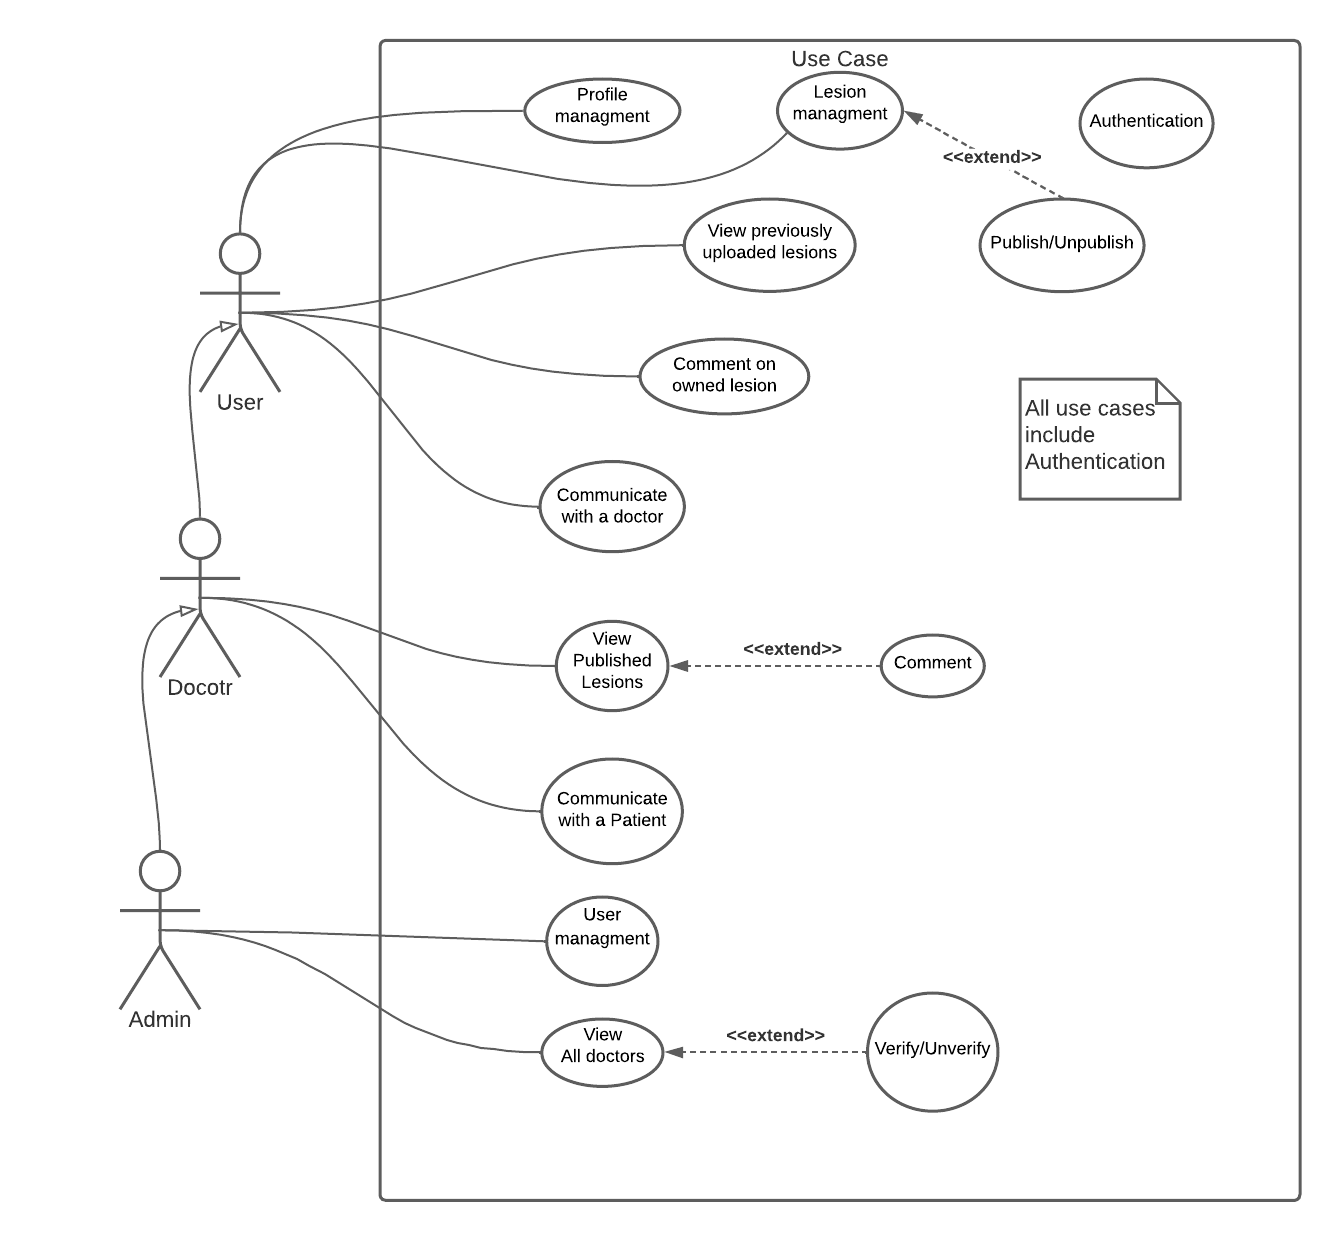
\includegraphics[width=18cm]{./diagnosis-system/conception/use-case.png}
\end{center}
\caption{Use Case Diagram}
\label{fig:}
\end{figure}



\subsection{Component Diagram}
An illustration of how components are linked together to create bigger components or software systems is called a component diagram. They serve as examples of how arbitrarily complex systems are structured.

\begin{figure}[H]
\begin{center}
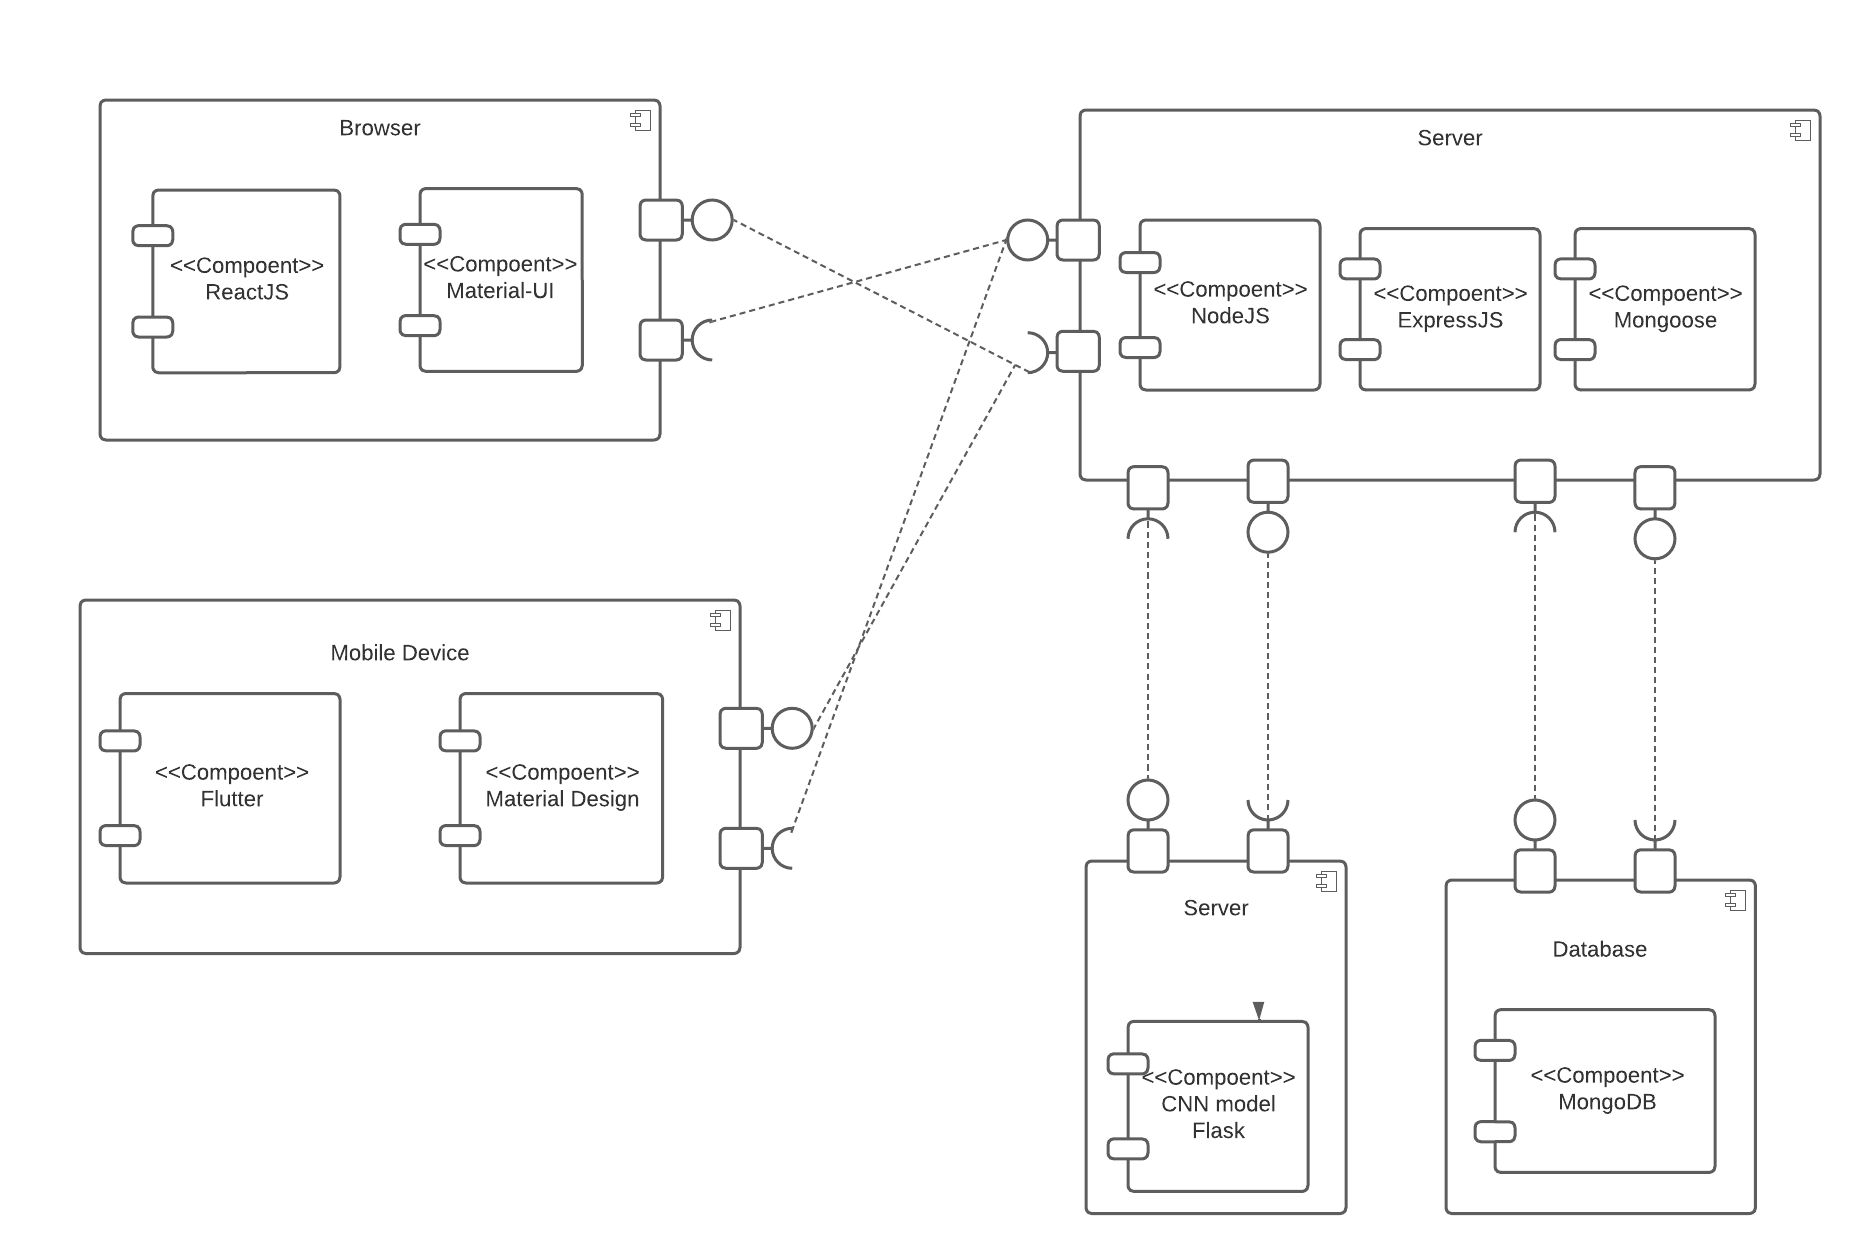
\includegraphics[width=18cm]{./diagnosis-system/conception/component.png}
\end{center}
\caption{Component Diagram}
\label{fig:}
\end{figure}

\subsection{Deployment Diagram}
A deployment diagram is a type of UML diagram that displays the system's execution architecture, including the middleware connecting the nodes—such as hardware or software execution environments—and the nodes themselves. Typically, deployment diagrams are used to illustrate a system's actual hardware and software.

\begin{figure}[H]
\begin{center}
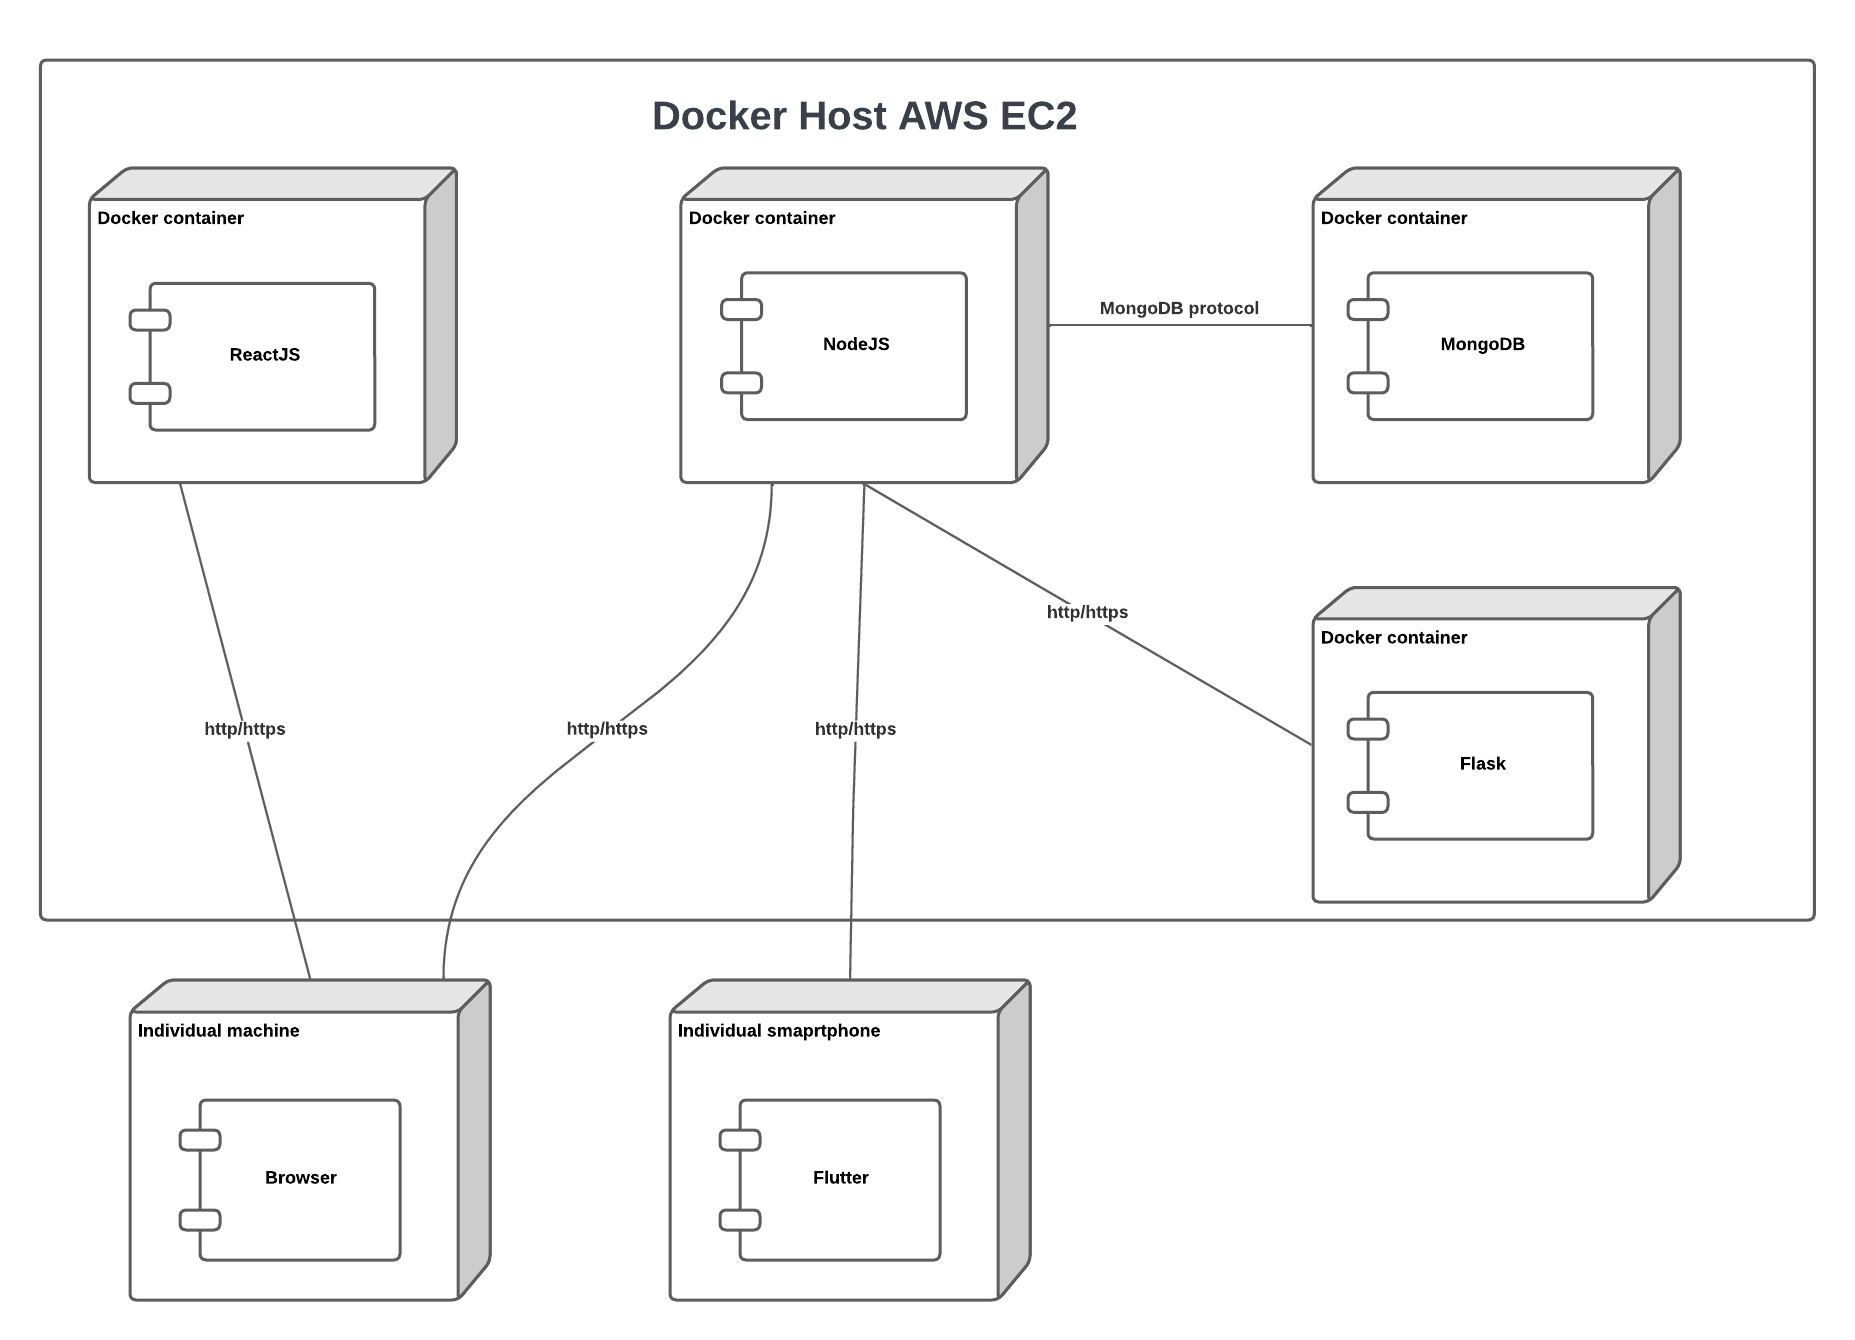
\includegraphics[width=18cm]{./diagnosis-system/conception/deployment.png}
\end{center}
\caption{Deployment Diagram}
\label{fig:dep}
\end{figure}

    
